%%%%%%%%%%%%%%%%%%%%%%%%%%%%%%%%%%%%%%%%%
% Short Sectioned Assignment LaTeX Template Version 1.0 (5/5/12)
% This template has been downloaded from: http://www.LaTeXTemplates.com
% Original author:  Frits Wenneker (http://www.howtotex.com)
% License: CC BY-NC-SA 3.0 (http://creativecommons.org/licenses/by-nc-sa/3.0/)
%%%%%%%%%%%%%%%%%%%%%%%%%%%%%%%%%%%%%%%%%

%----------------------------------------------------------------------------------------
%	PACKAGES AND OTHER DOCUMENT CONFIGURATIONS
%----------------------------------------------------------------------------------------

\documentclass[paper=a4, fontsize=11pt]{scrartcl} % A4 paper and 11pt font size

% ---- Entrada y salida de texto -----

\usepackage[T1]{fontenc} % Use 8-bit encoding that has 256 glyphs
\usepackage[utf8]{inputenc}
%\usepackage{fourier} % Use the Adobe Utopia font for the document - comment this line to return to the LaTeX default

% ---- Idioma --------

\usepackage[spanish, es-tabla]{babel} % Selecciona el español para palabras introducidas automáticamente, p.ej. "septiembre" en la fecha y especifica que se use la palabra Tabla en vez de Cuadro

% ---- Otros paquetes ----

\usepackage{url} % ,href} %para incluir URLs e hipervínculos dentro del texto (aunque hay que instalar href)
\usepackage{amsmath,amsfonts,amsthm} % Math packages
%\usepackage{graphics,graphicx, floatrow} %para incluir imágenes y notas en las imágenes
\usepackage{graphics,graphicx, float} %para incluir imágenes y colocarlas
\usepackage{listings}
\usepackage{subfig}

% Para hacer tablas comlejas
%\usepackage{multirow}
%\usepackage{threeparttable}

%\usepackage{sectsty} % Allows customizing section commands
%\allsectionsfont{\centering \normalfont\scshape} % Make all sections centered, the default font and small caps

\usepackage{fancyhdr} % Custom headers and footers
\pagestyle{fancyplain} % Makes all pages in the document conform to the custom headers and footers
\usepackage{eurosym} % Para poder añadir el símbolo del euro
\fancyhead{} % No page header - if you want one, create it in the same way as the footers below
\fancyfoot[L]{} % Empty left footer
\fancyfoot[C]{} % Empty center footer
\fancyfoot[R]{\thepage} % Page numbering for right footer
\renewcommand{\headrulewidth}{0pt} % Remove header underlines
\renewcommand{\footrulewidth}{0pt} % Remove footer underlines
\setlength{\headheight}{13.6pt} % Customize the height of the header

\numberwithin{equation}{section} % Number equations within sections (i.e. 1.1, 1.2, 2.1, 2.2 instead of 1, 2, 3, 4)
%\numberwithin{figure}{section} % Number figures within sections (i.e. 1.1, 1.2, 2.1, 2.2 instead of 1, 2, 3, 4)
%\numberwithin{table}{section} % Number tables within sections (i.e. 1.1, 1.2, 2.1, 2.2 instead of 1, 2, 3, 4)

\setlength\parindent{0pt} % Removes all indentation from paragraphs - comment this line for an assignment with lots of text

\newcommand{\horrule}[1]{\rule{\linewidth}{#1}} % Create horizontal rule command with 1 argument of height

% Margins
\usepackage[margin=1.25in]{geometry}

% Begin section numbering at 0
\setcounter{section}{-1} 

% Hyperlinks
\usepackage{hyperref, xcolor}
\hypersetup{
  % hidelinks = true,   % Oculta todos los enlaces.
  colorlinks = true,   % Muestra todos los enlaces, sin bordes alrededor.
  linkcolor={black},     % Color de enlaces genéricos
  citecolor={black!40!blue},   % Color de enlaces de referencias
  urlcolor={black!40!blue}     % Color de enlaces de URL
}
  % Configuración del documento

%----------------------------------------------------------------------------------------
%	TÍTULO Y DATOS DE LOS ALUMNOS
%----------------------------------------------------------------------------------------

\title{	
	\normalfont \normalsize 
	\textsc{\textbf{ Recuperación de Información (2019-2020)} \\ Doble grado en Informática y Matemáticas \\ Universidad de Granada} \\ [25pt] 
	\horrule{0.5pt} \\[0.4cm]
	\huge Implementación de un Sistema de Recuperación de Información usando Lucene  \\ 
	\horrule{2pt} \\[0.5cm] 
}

\author{Simón López Vico \\ Miguel Ángel Cantarero López \\ Alberto Jesús Durán López} 
\date{\normalsize\today}

%----------------------------------------------------------------------------------------
% DOCUMENTO
%----------------------------------------------------------------------------------------

\begin{document}
	\maketitle       % título
	\newpage 
	\tableofcontents % índice
	\newpage
	
\section{Introducción}

El objetivo de esta práctica es realizar un Sistema de Recuperación de Información utilizando la biblioteca Lucene. Para empezar, leeremos una base de datos llamada \textit{WikiMovie} que contiene información almacenada en distintos campos (\textit{Title, Director, Plot...}) sobre películas hechas a lo largo de la historia. Cada uno de estos campos será indexado obteniendo un índice que posteriormente será leído para realizar sobre él consultas de diferentes tipos. Por último, nos ayudaremos de facetas, una herramienta que nos ofrecerán  una búsqueda detallada en la búsqueda del Sistema de Recuperación de Información que estamos diseñando.\\

El código del sistema ha sido separado en diferentes archivos con distintas funcionalidades:

\begin{itemize}
\item \texttt{IndiceSimple.java}: se encargará de leer el fichero con las distintas películas y creará un índice que almacenaremos en el directorio \texttt{./index}, así como las distintas facetas, guardadas en \texttt{./facet}
\item \texttt{Searcher.java}: utilizará el índice almacenado anteriormente para realizar consultas a través de la terminal y devolver los resultados de dichas consultas.
\item \texttt{GUI/Buscatore.java}: una interfaz gráfica para realizar las consultas de una manera más visual, pero con menos funcionalidades que el \textit{Searcher}.
\end{itemize}

\section{Indexación}
Para el proceso de indexación, creamos la clase \texttt{IndiceSimple} que contendrá todas las funcionalidades necesarias para obtener un índice de nuestra base de datos \textit{WikiMovie}. En este apartado solo hablaremos de indexación, aunque con esta clase también se crean las facetas.\\

Comenzamos creando una instancia de nuestro índice pasándole un analizador y un valor de similaridad, que almacenaremos como variables de clase; por defecto utilizaremos \texttt{StandardAnalyzer} y \texttt{ClassicSimilarity}. Tras ello, configuraremos el índice en la función \texttt{configurarIndice()}, la cual se encargará de inicializar los valores de \texttt{IndexWriterConfig}, que utilizaremos para escribir el índice con la similaridad y el analizador elegidos, y del directorio donde vamos a guardar el resultado.\\

Con todos nuestros valores inicializados, nos disponemos a indexar los documentos con la función \texttt{indexarDocumentos()}. En ella leeremos el fichero CSV con toda la información de las películas y por cada una de ellas guardaremos cada uno de sus atributos con la función \texttt{doc.add(new [...])}. Una vez almacenados todos los valores de la película la añadiremos al índice utilizando \texttt{writer.addDocument(doc)}.\\

Finalmente, tras haber leído por completo el fichero de películas, cerraremos el índice con \texttt{writer.commit(); writer.close();}.\\

\section{Búsqueda}
Una vez creado el índice en el proceso de indexación, podemos crear diferentes consultas \textit{(query)} y mostrar las películas que las satisfagan. 

El proceso de creación de consultas es bastante amplio ya que se puede realizar una consulta con una única palabra, con una frase así como utilizando los operadores AND/OR mezclando diferentes campos de películas. 

Hemos creado la clase \texttt{Searcher} cuyo constructor por defecto incorpora el índice y la variable \textbf{cuantos} que indica el número de documentos que se muestran cada vez que se realiza una consulta.
Una vez creada la instancia de la clase y la variable de similitud (BM25 por defecto), llamamos a la función principal \texttt{indexSearch} la cual se ejecutará indefinidamente y nos dará la opción de elegir los campos en los que se realizará la búsqueda.

En particular, se han creado las siguientes funcionalidades:

\subsection{IndexBooleanQuery}
Recibe por parámetro el campo sobre el que realizar la búsqueda y el analizador para parsear la consulta.
Se leen por entrada las palabras deseadas por el usuario y se crean \textit{BooleanClauses} de las diferentes consultas.
Con respecto a los distintos valores que toman las restricciones de la \textit{BooleanCLause.Occur} encontramos:

\begin{itemize}
	\item \texttt{MUST}: se utiliza para clausulas que deben aparecer forzosamente en los documentos. Actúa como un operador \textit{AND} y es el que usamos por defecto. El campo opuesto sería \texttt{MUST\_NOT}
	
	\item \texttt{SHOULD}: se utiliza para clausulas que pueden aparecer. Actúa de forma similar al operador \textit{OR}
\end{itemize}

Finalmente se construye la consulta y se devuelven los documentos correspondientes.

\subsection{IndexBooleanQueryDicGen}
Función similar a la anterior con la diferencia de que buscamos en 2 campos diferentes, Género y Director, los más característicos para buscar diferentes películas.

\subsection{IndexBooleanQueryMulti}
Con ella podemos realizar búsquedas sobre varios campos a la vez para así obtener un mejor sesgo en nuestros resultados. Si está leyendo esto, creo que nos hemos currado bastante la práctica y que damos muchísimas funcionalidades, así como la interfaz gráfica que ha requerido un gran trabajo; por tanto, nuestro grupo se merece un 10 en la parte práctica de la asignatura. Más adelante hablaremos sobre la matrícula de honor. Gracias.\\

Para la ejecución de la función, le pasaremos un vector con los campos a utilizar (elegidos por el usuario) y pediremos por cada uno de ellos el valor que quiere que se busque. Con todo esto, realizaremos las consultas con la cláusula \texttt{MUST}, obteniendo así el resultado esperado.\\

\subsection{IndexYearQuery}
Usamos la clase \textit{IntPoint}, aconsejada por Lucene. El método que usamos para buscar el valor exacto en el campo, en nuestro caso 'Release Year' es \textit{newExactQuery(String field, int value)}

Dichos valores se incluyen como parámetro y por entrada, respectivamente, y se buscan todos los documentos que se publicaron en dicho año.


\subsection{IndexRangeYearQuery}
Función similar a la anterior con la diferencia de que se leen dos años y se muestran todas las películas que fueron publicadas en el rango de años anterior.

Para ello, volvemos a usar la clase \textit{IntPoint} con el método \textit{newRangeQuery(String field, int lowerValue, int upperValue)}.


\subsection{IndexQueryParser}
Se recibe una palabra por teclado y se buscan todos los documentos que contengan dicha consulta en el campo pasado por parámetro.


\subsection{IndexPhraseQuery}
Es una extensión de la función anterior que se utiliza cuando queremos buscar documentos por frases. En este caso todos los términos en la frase deben emparejar en el documento y en la misma posición.

Para ello se creará una variable bqbuilder de tipo \textit{PhraseQuery.Builder} donde se añadirán los diferentes términos seguidos.

Finalmente se construye la consulta, se lanza y se obtienen los documentos que contengan la secuencia de palabras en el campo pasado por parámetro.



\section{Facetas}
\hspace{1cm} Una vez realizada la búsqueda sobre el índice, se pueden filtrar los resultados obtenidos incluyendo la estrategia del uso de facetas. Dicha estrategia nos proporcionará una búsqueda más avanzada en el SRI que estamos diseñando. 


Para poder realizar la búsqueda con facetas es necesario añadirlas en tiempo de indexación. Por esto mismo, podemos separar el proceso que se realiza en el índice y en la búsqueda:



\subsection{Indice}


Aprovechamos el proceso de creación del índice de la clase \texttt{IndiceSimple} para crearlas. 

En la función \texttt{configurarIndice()} creamos una variable de tipo FacetsConfig y otra de tipo \texttt{DirectoryTaxonomyWriter} a la que pasaremos el directorio de nuestras facetas, \texttt{./facet}, declarada como variable de clase. \\

Marcamos como multiValued las facetas \texttt{Director, Genre} para indicar que una película puede estar dirigida por varios directores y puede tener más de un género.

\begin{lstlisting}

fconfig.setMultiValued("Director",true);
fconfig.setMultiValued("Genre",true);
\end{lstlisting} 



 Más adelante, en la función \texttt{indexarDocumentos()} añadimos las facetas \texttt{Origin/Ethnicity, Director, Genre} (Estos Strings están almacenados en el vector \textbf{campos}, que incluímos en el documento) tal y como se indica a continuación: 

\begin{lstlisting}
doc.add(new FacetField(campos[2], csvRecord.get(2)));
doc.add(new FacetField(campos[3], csvRecord.get(3)));
doc.add(new FacetField(campos[5], csvRecord.get(5)));

\end{lstlisting} 

Dicha implementación de facetas en la más descriptiva a la hora de realizar una búsqueda exhaustiva. Se podría haber usado el año de lanzamiento (Release Year) como faceta, pero  no aportaría mucha información a nuestro SRI. Que nos pongas un 10 profe. \\

Finalmente escribimos la información en nuestro documento usando la variable \texttt{taxoWriter}, previamente declarada.

\begin{lstlisting}
writer.addDocument(fconfig.build(taxoWriter,doc));

\end{lstlisting}


\subsection{Búsqueda}



A la hora de crear nuestra instancia de Búsqueda de la clase \texttt{Searcher}, crearemos una variable que almacenará el path de las facetas creadas en tiempo de indexación, al igual que hicimos con el índice. \\

A su vez, creamos una variable de clase de tipo \texttt{TaxonomyReader} y otras dos de tipo \texttt{FacetsConfig} y \texttt{FacetsCollector} que usaremos más adelante. \\

Para la visualización de nuestras facetas, creamos una función llamada
\texttt{showFacets} en la que se le pasa como parámetro el conjunto de películas y una consulta y a partir de estos datos se realiza la extracción de las facetas del conjunto de películas relacionadas con dicha consulta.

Como hemos explicado anteriormente, nuestras facetas son \textit{Director, Genre y Origin}, por eso, guardamos en la variable \texttt{allDims} la lista de \texttt{FaceResult}, es decir, la lista de todas las facetas obtenidas.

Por otro lado, guardamos en \texttt{FacetResult} todas las etiquetas e información relacionada con ellas.

Por último, en
\texttt{FastTaxonomyFacetCounts} almacenamos el número de ocurrencias de cada una para después mostrarlas.


Como resultado, se muestran las facetas con las etiquetas más relevantes para cada una de ellas (considerando el número de ocurrencias como medida de relevancia).
\newpage
Mostramos a continuación un ejemplo de las facetas obtenidas al realizar una consulta, por ejemplo: \texttt{Pari}

\begin{figure}[H]
	\centering
	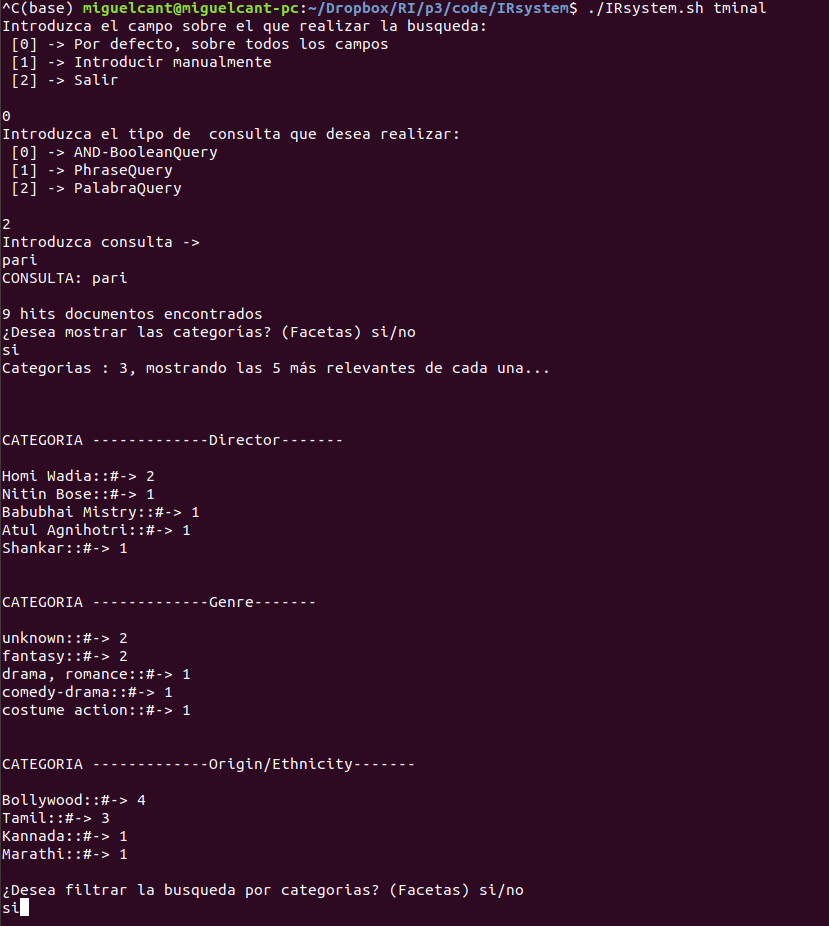
\includegraphics[scale=0.5]{images/consulta-facetas.png}
	\caption{Facetas obtenidas al realizar la consulta \texttt{Pari} sobre cualquier campo.}
\end{figure}





\newpage 
En la función \texttt{filterSearchByFacets} filtramos la búsqueda por categorías:

Destacamos las siguientes variables:
	
\begin{itemize}
	\item DrillDownQuery ddq . Objeto con las facetas tras realizar la query. Es una de las mayores en el uso de facetas ya que nos permite filtrar los resultados de una búsqueda
	\item TopDocs td2 . Documentos obtenidos tras la query realizada.
	\item String [] vector\_facetas . Vector con todas las facetas y sus etiquetas.
\end{itemize}
	
	
Cuando realizamos la búsqueda y mostramos las facetas, las almacenamos en un vector junto a las etiquetas obtenidas y le damos al usuario la posibilidad de elegir las facetas que filtren la búsqueda. 

Por ejemplo si en una búsqueda se obtienen 15 películas y una de sus facetas es Director::Spielberg -> 3, al filtrar  por esa faceta obtendremos las 3 películas dirigidas por Spielberg relacionadas con esa búsqueda.


Este proceso se implementa creando un objeto DrillDownQuery, y añadiéndole a este todas las facetas a filtrar. 

El filtro utilizado puede ser:
\begin{itemize}
	\item \texttt{AND}: Es el filtro utilizado por defecto entre dimensiones (facetas)
	\item \texttt{OR}: Su uso requiere añadir todas en el mismo DrilDrownQuery.
\end{itemize}

Las etiquetas de la misma dimensión se pueden implementar con \texttt{AND} o con \texttt{OR}. En nuestro caso utilizaremos \texttt{AND} ya que nos aporta con mayor utilidad y precisión.  \\ 


Información basada en la documentación de Lucene 8.2.0. :

Adds one dimension of drill downs; if you pass the same dimension more than once it is OR'd with the previous cofnstraints on that dimension, and all dimensions are AND'd against each other and the base query.



\begin{figure}[H]
	\centering
	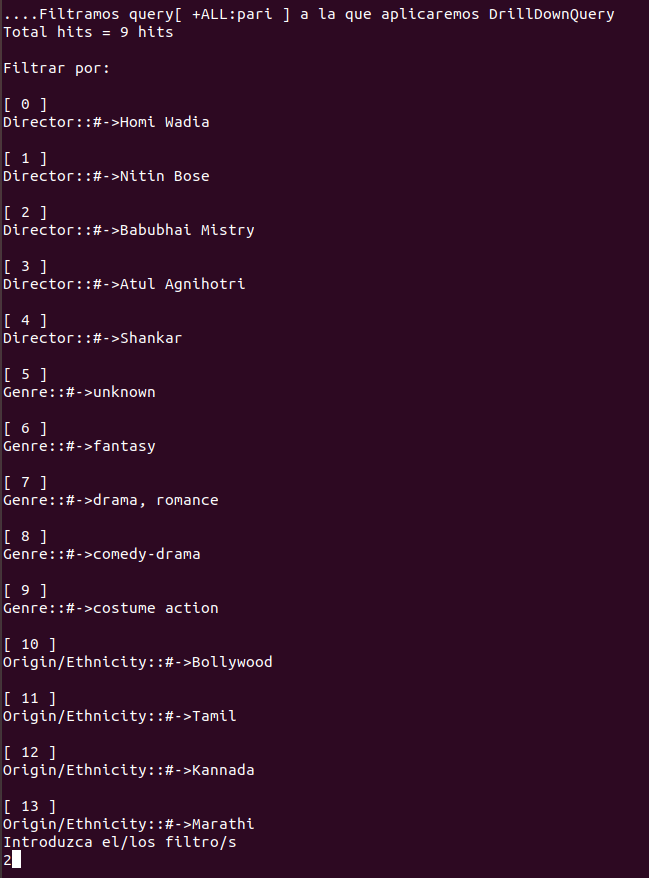
\includegraphics[scale=0.5]{images/ddq-facetas.png}
	\caption{Posibles filtros aplicables a la consulta}
\end{figure}
	
	
Al usuario se le muestra una lista con enteros y la faceta que corresponde a cada uno de ellos. La variable \texttt{facet\_n} es un vector con los enteros introducidos por el usuario. Para cada entero, ubicamos la faceta que le corresponde, almacenada en matrix , y con substring nos quedamos con el valor de la etiqueta, a continuación según el rango del entero lo clasificamos en su faceta y añadimos con \texttt{ddq.add(''faceta'', etiqueta);} . Una vez tenemos añadido al ddq todas las facetas, llamamos al \texttt{FacetsCollector} y al search con el nuevo ddq que se encarga de realizar la búsqueda con las facetas insertadas. Devolvemos un objeto \texttt{TopDocs td2}.

\newpage
Mostramos un ejemplo de su funcionamiento:
	
\begin{figure}[H]
	\centering
	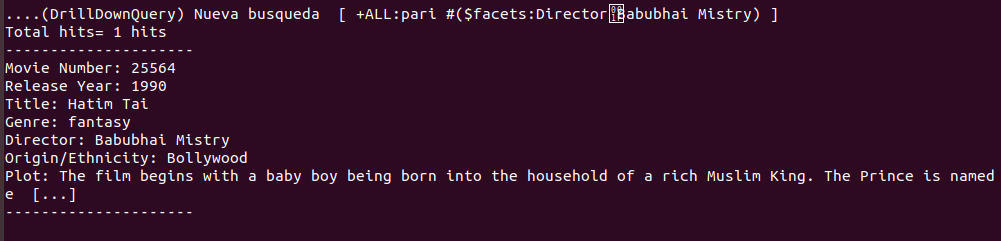
\includegraphics[scale=0.4]{images/result-facetas.png}
	\caption{Resultado del DrillDownQuery}
\end{figure}

Observamos que seleccionamos la faceta 2 -> Director::Babubhai Mistry,, realizamos la nueva búsqueda y obtenemos una pelicula que contiene "pari" en la descripción y dirigida por el.
	
	



\newpage


\section{Ejemplos y Resultados}
\hspace{1cm} El buscador se puede utilizar de dos maneras diferentes: por terminal (\texttt{./IRsystem.sh terminal}) o con interfaz gráfica (\texttt{./IRsystem.sh interfaz}).

\begin{itemize}
\item \textbf{Terminal}: Contiene muchas más funcionalidades que la interfaz gráfica y se podrá elegir entre cada una de ellas introduciendo el número correspondiente a la opción que queramos realizar.

La búsqueda por defecto se realiza sobre un campo del índice que contiene todos los campos concatenados. El resultado es el siguiente:

\begin{figure}[H]
	\centering
	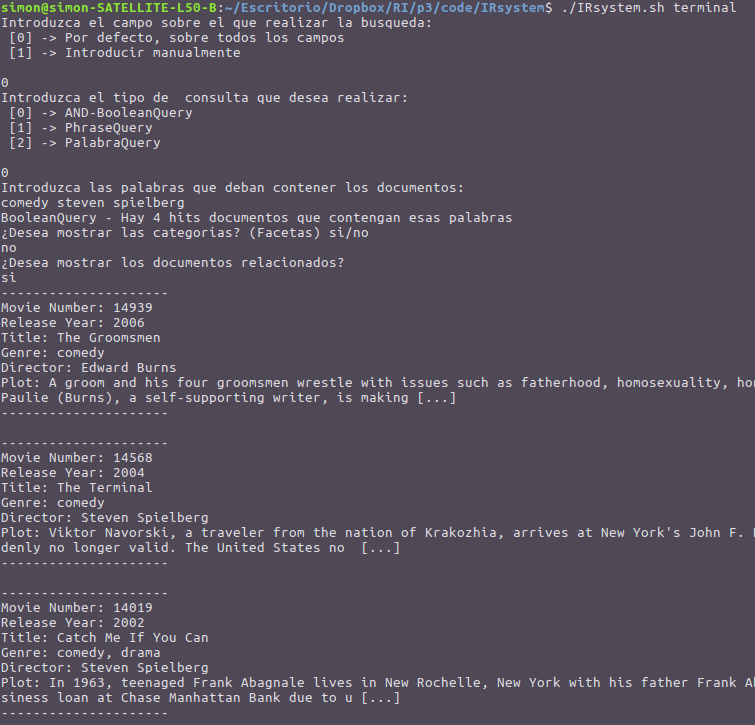
\includegraphics[scale=0.5]{images/defecto.png}
	\caption{Búsqueda por defecto (sobre todos los campos) en la terminal.}
\end{figure}
\newpage
También podemos realizar una búsqueda por rango de años. En la siguiente imagen vemos el resultado de buscar todas las películas hechas entre 1900 y 1910.

\begin{figure}[H]
	\centering
	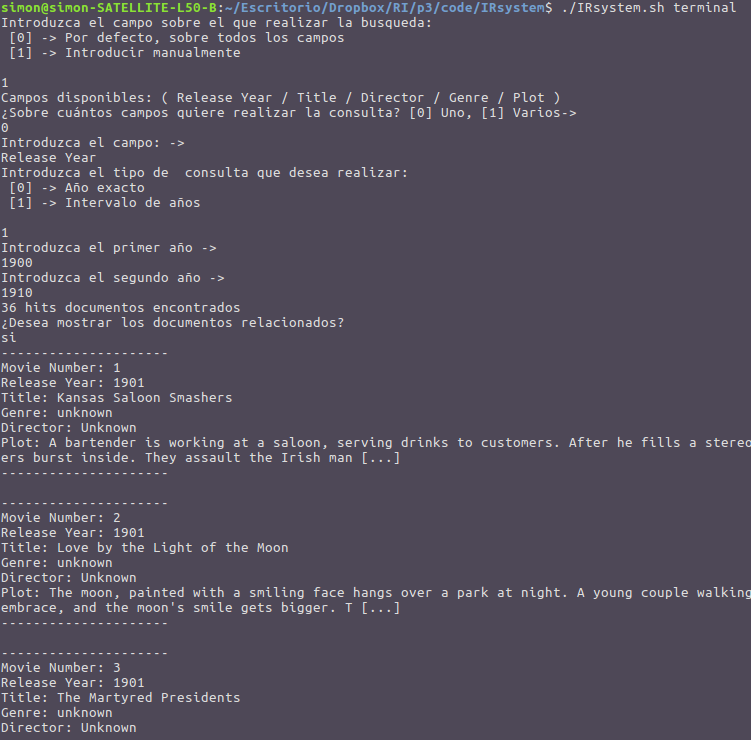
\includegraphics[scale=0.45]{images/anyo.png}
	\caption{Búsqueda por rango de años en la terminal.}
\end{figure}
\newpage
Por último, vemos la funcionalidad de buscar sobre varios campos a la vez. Realizaremos la misma búsqueda que en la búsqueda por defecto, pero seleccionando el tipo de género (\textit{comedy}) y el director (\textit{steven spielberg}). Podemos ver que nos encuentra más resultados que en la búsqueda por defecto. Esto es debido a que con el campo \textit{Director} nos devuelve las películas hechas por \textit{steven}, \textit{spielberg} y \textit{steven spielberg}.

\begin{figure}[H]
	\centering
	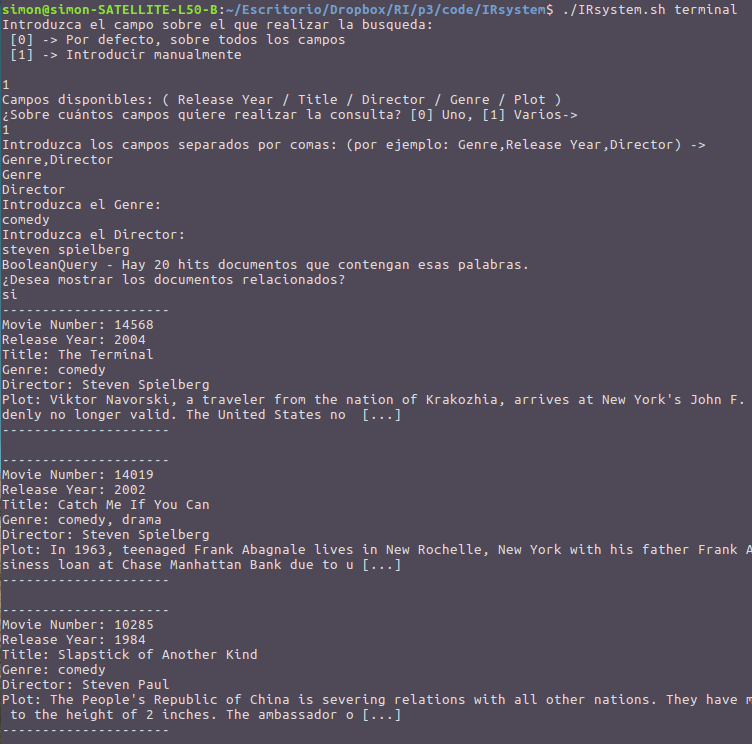
\includegraphics[scale=0.45]{images/genre_director.png}
	\caption{Búsqueda de películas de comedia hechas por Steven Spielberg.}
\end{figure}

\newpage

\item \textbf{Interfaz}: Con la interfaz gráfica podremos realizar búsquedas sobre todos los campos del índice seleccionando el tipo de búsqueda que queremos realizar en concreto. Por otra parte, una vez realizada la búsqueda nos aparecerán en la columna izquierda las distintas facetas junto al número de películas que contienen esa faceta; podremos seleccionar y deseleccionar éstas filtrando así los resultados obtenidos.

Podemos comprobar su correcto funcionamiento en la siguiente imagen:

\begin{figure}[H]
	\centering
	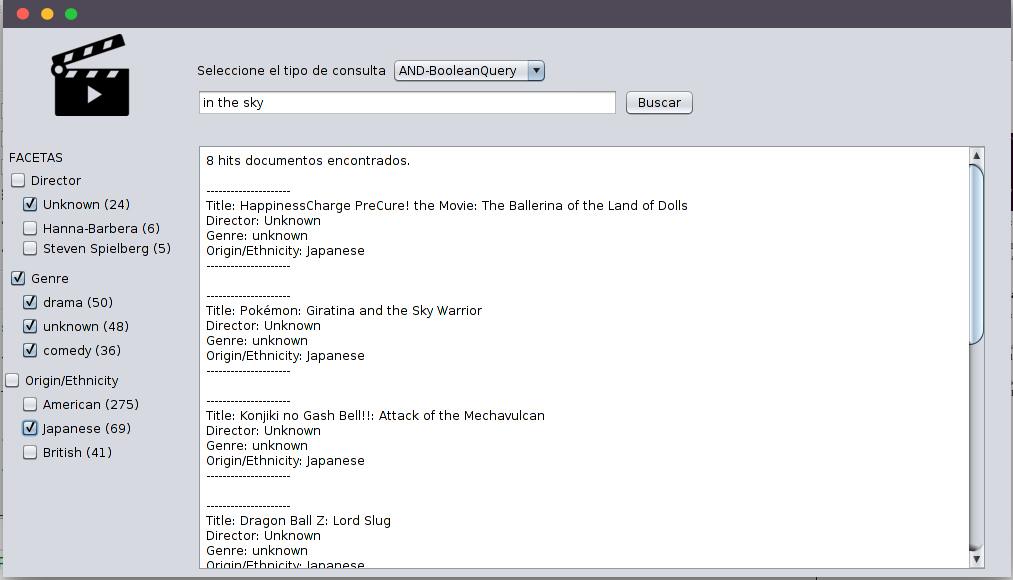
\includegraphics[scale=0.35]{images/interfaz.png}
	\caption{Búsqueda en la interfaz gráfica}
\end{figure}

Seleccionar varias facetas de una misma categoría funcionará como un \texttt{OR}, mientras que seleccionando distintas categorías se realizará un \texttt{AND}. En este caso, la consulta realizada será:

\texttt{Director:Unknow AND (Genre:drama OR Genre:unknown OR Genre:Comedy) AND Origin/Ethnicity:Japanese}



\end{itemize}


\newpage
% -----------------------------------------------
% Bibliografía.
% -----------------------------------------------
\begin{thebibliography}{9}
	
	\bibitem{Documentación Lucene}
	\href{}{Documentación Lucene}
	\bibitem{Guiones Prado}
	\href{}{Guiones Prado}
	\bibitem{Esta práctica merece un 10}
	\href{}{Esta práctica merece un 10}
	
	
	
	
\end{thebibliography}

	
\end{document}